% The keys the global random state derives for a short program: every sampling
% call splits the state at its counter, nv_while() forks a child state, and a
% key is either split or drawn from, never both.
% Build: see figures/README.md
\documentclass[tikz, border = 6pt]{standalone}
\usepackage[T1]{fontenc}
\usepackage{lmodern}
\usepackage{amsmath}
\usetikzlibrary{positioning, calc, arrows.meta, fit, backgrounds}

\definecolor{hash}{HTML}{5B8C5A}
\definecolor{keep}{HTML}{2A7AB0}
\definecolor{fork}{HTML}{E08A2C}

\tikzset{
  >={Stealth[length = 2mm]},
  state/.style = {draw, rounded corners = 2pt, inner sep = 4pt, align = center,
    font = \small},
  key/.style = {draw = hash!80!black, fill = hash!15, rounded corners = 2pt,
    inner sep = 3pt, font = \small, minimum height = 6mm},
  forkkey/.style = {key, draw = fork!80!black, fill = fork!15},
  bits/.style = {draw = keep!80!black, fill = keep!15, inner sep = 2.5pt,
    font = \footnotesize, minimum height = 5mm},
  code/.style = {font = \ttfamily\footnotesize, text = black!65, anchor = south west,
    inner sep = 1pt},
  edge/.style = {->, black!70},
  elabel/.style = {font = \footnotesize, fill = white, inner sep = 1pt}
}

\begin{document}
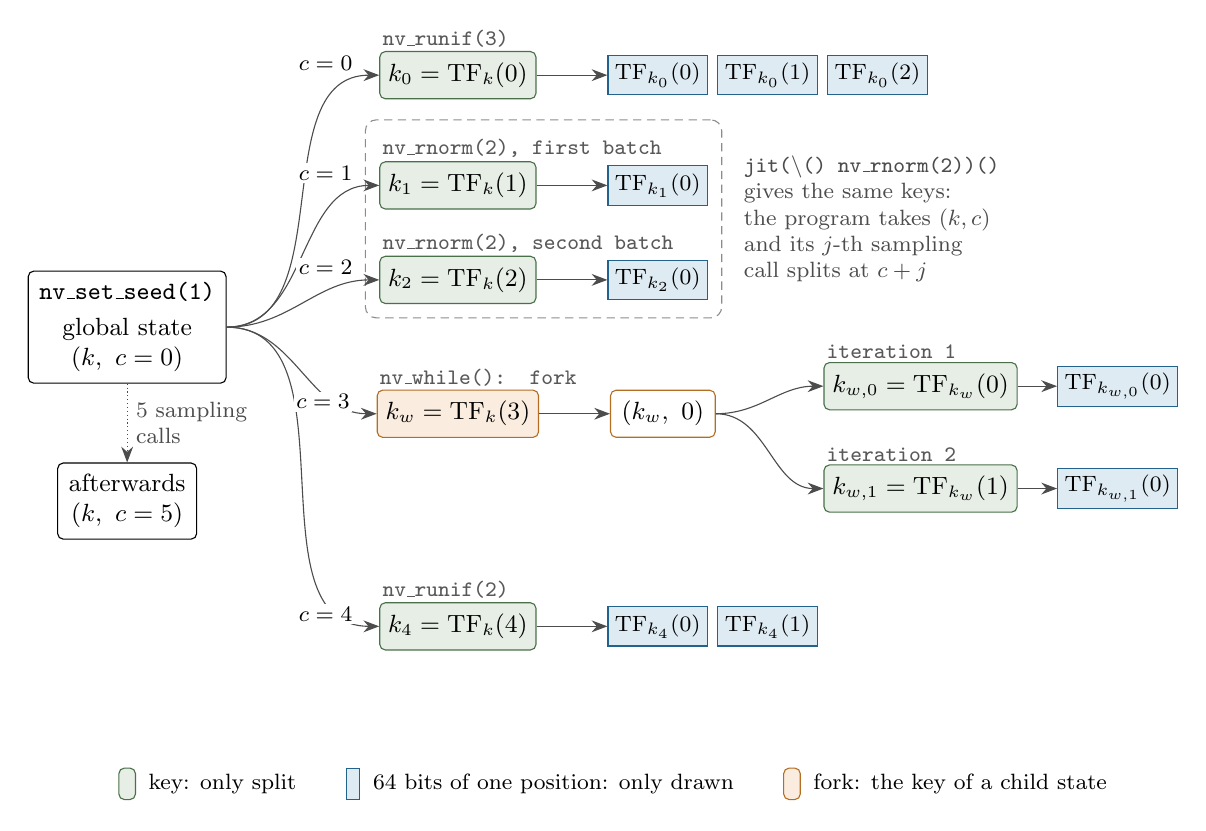
\begin{tikzpicture}

  % ---- the global random state --------------------------------------------
  \node[state] (root) at (0, -3.2)
    {\texttt{nv\_set\_seed(1)}\\[2pt]global state\\$(k,\ c = 0)$};

  % ---- one split per sampling call ----------------------------------------
  \foreach \c/\y/\name in {0/0/k0, 1/-1.4/k1, 2/-2.6/k2, 4/-7.0/k4} {
    \node[key] (\name) at (4.2, \y) {$k_{\c} = \mathrm{TF}_k(\c)$};
    \draw[edge] (root.east) to[out = 0, in = 180] (\name.west);
    \node[elabel, anchor = south east] at ($(\name.west) + (-0.3, 0.02)$) {$c = \c$};
  }
  \node[forkkey] (k3) at (4.2, -4.3) {$k_w = \mathrm{TF}_k(3)$};
  \draw[edge] (root.east) to[out = 0, in = 180] (k3.west);
  \node[elabel, anchor = south east] at ($(k3.west) + (-0.3, 0.02)$) {$c = 3$};

  \node[code] at (k0.north west) {nv\_runif(3)};
  \node[code] at (k1.north west) {nv\_rnorm(2), first batch};
  \node[code] at (k2.north west) {nv\_rnorm(2), second batch};
  \node[code] at (k3.north west) {nv\_while(): fork};
  \node[code] at (k4.north west) {nv\_runif(2)};

  % ---- draws: one block per position t ------------------------------------
  \node[bits, right = 0.9 of k0] (b00) {$\mathrm{TF}_{k_0}(0)$};
  \node[bits, right = 0.12 of b00] (b01) {$\mathrm{TF}_{k_0}(1)$};
  \node[bits, right = 0.12 of b01] (b02) {$\mathrm{TF}_{k_0}(2)$};
  \draw[edge] (k0) -- (b00);

  \node[bits, right = 0.9 of k1] (b10) {$\mathrm{TF}_{k_1}(0)$};
  \draw[edge] (k1) -- (b10);
  \node[bits, right = 0.9 of k2] (b20) {$\mathrm{TF}_{k_2}(0)$};
  \draw[edge] (k2) -- (b20);

  \node[bits, right = 0.9 of k4] (b40) {$\mathrm{TF}_{k_4}(0)$};
  \node[bits, right = 0.12 of b40] (b41) {$\mathrm{TF}_{k_4}(1)$};
  \draw[edge] (k4) -- (b40);

  % ---- the loop body's own random state -----------------------------------
  \node[state, draw = fork!80!black, right = 0.9 of k3] (child) {$(k_w,\ 0)$};
  \draw[edge] (k3) -- (child);
  \node[key] (w0) at ($(child.east) + (2.6, 0.35)$) {$k_{w,0} = \mathrm{TF}_{k_w}(0)$};
  \node[key] (w1) at ($(child.east) + (2.6, -0.95)$) {$k_{w,1} = \mathrm{TF}_{k_w}(1)$};
  \draw[edge] (child.east) to[out = 0, in = 180] (w0.west);
  \draw[edge] (child.east) to[out = 0, in = 180] (w1.west);
  \node[code] at (w0.north west) {iteration 1};
  \node[code] at (w1.north west) {iteration 2};
  \node[bits, right = 0.5 of w0] (bw0) {$\mathrm{TF}_{k_{w,0}}(0)$};
  \node[bits, right = 0.5 of w1] (bw1) {$\mathrm{TF}_{k_{w,1}}(0)$};
  \draw[edge] (w0) -- (bw0);
  \draw[edge] (w1) -- (bw1);

  % ---- jit: the same keys --------------------------------------------------
  \coordinate (jittop) at ($(k1.north west) + (0, 0.35)$);
  \begin{scope}[on background layer]
    \node[draw = black!45, densely dashed, rounded corners = 4pt, inner sep = 5pt,
      fit = (k1) (k2) (b10) (b20) (jittop)] (jitbox) {};
  \end{scope}
  \node[font = \footnotesize, align = left, anchor = west, text = black!70]
    at ($(jitbox.east) + (0.15, 0)$)
    {\texttt{jit(\textbackslash() nv\_rnorm(2))()}\\gives the same keys:\\the program takes $(k, c)$\\and its $j$-th sampling\\call splits at $c + j$};

  % ---- afterwards -----------------------------------------------------------
  \node[state, below = 1.0 of root] (after) {afterwards\\$(k,\ c = 5)$};
  \draw[edge, densely dotted] (root) -- node[elabel, right = 2pt, align = left] {5 sampling\\calls} (after);

  % ---- legend ---------------------------------------------------------------
  \node[key, minimum height = 4mm] (lk) at (0, -9.0) {};
  \node[right = 1pt of lk, font = \footnotesize] (lkt) {key: only split};
  \node[bits, minimum height = 4mm, right = 0.5 of lkt] (lb) {};
  \node[right = 1pt of lb, font = \footnotesize] (lbt) {64 bits of one position: only drawn};
  \node[forkkey, minimum height = 4mm, right = 0.5 of lbt] (lf) {};
  \node[right = 1pt of lf, font = \footnotesize]
    {fork: the key of a child state};

\end{tikzpicture}
\end{document}
